\documentclass{beamer}

\usepackage[utf8]{inputenc}
\usepackage[T1]{fontenc}
\usepackage[ngerman]{babel}
\usepackage{graphicx} % Bilder
\usepackage{wrapfig} % Umflussbilder
\usepackage{multicol} % Multiple columns
\usepackage{minted} % Haskell source code
\usepackage{framed} % Frames around source code
\usepackage[framemethod=tikz]{mdframed} % Frames
\usepackage{verbatim} % \begin{comment}...\end{comment}
\usepackage{etoolbox} % manipulate minted
\AtBeginEnvironment{minted}{\fontsize{10}{10}\selectfont}
\AfterEndEnvironment{minted}{}

\mdfdefinestyle{fancy}{
  roundcorner=5pt,
  linewidth=4pt,
  linecolor=red!80,
  backgroundcolor=red!20
}
\newmdenv[style=fancy]{important}

% redifine \em for \emph to use bold instead of italics
\makeatletter
\DeclareRobustCommand{\em}{%
  \@nomath\em \if b\expandafter\@car\f@series\@nil
  \normalfont \else \bfseries \fi}
\makeatother

% Stuff for Beamer
\beamertemplatenavigationsymbolsempty
\usetheme{Warsaw}

\title{Fortgeschrittene Funktionale Programmierung in Haskell}

\begin{document}

%  \usebackgroundtemplate{\includegraphics[width=\paperwidth,height=\paperheight]{1.jpg}} 
  
%----------------------------------------------------------------------------------------  

  \begin{frame}
  \begin{center}
    \huge\textbf{Fortgeschrittene Funktionale Programmierung in Haskell}\\ \bigskip
    \LARGE Universität Bielefeld, Sommersemester 2015\\ \bigskip
    \large Jonas Betzendahl \& Stefan Dresselhaus
    \end{center}
  \end{frame}

%----------------------------------------------------------------------------------------  
\begin{frame}[allowframebreaks]{Outline}
\frametitle{Übersicht}
\tableofcontents[hideallsubsections]
\end{frame}

\begin{frame}
Worum soll es heute gehen?
\begin{itemize}
 \item Funktionale Programmierung generell
 \pause
 \item Implementierung einer Double-Linked-List\\
       Wie macht man sowas in Haskell?
 \pause
 \item Lazyness\\
       Was für Auswirkungen hat das auf die Programmierung?\\
       Was für Möglichkeiten bietet dies?
\end{itemize}

\end{frame}


\section{Double-Linked List}

\subsection{Anforderungen}

\begin{frame}
Eine Double-Linked-List ist die klassische Einstiegs-Datenstruktur in der imperativen Welt.\\\par \pause
Sie besteht aus
\begin{itemize}
 \item Einem Paar von Pointern, die auf den Anfang und das Ende zeigen
 \pause
 \item Aus Elementen, welche bestehen aus
 \pause
 \begin{itemize}
  \item Einem Pointer auf das nächste Element (null, falls nicht da)
  \pause
  \item Einem Pointer auf das vorherige Element (null, falls nicht da)
  \pause
  \item Einem Datum, welches gespeichert werden soll
 \end{itemize}

\end{itemize}

\end{frame}

\begin{frame}
Grafisch:
\begin{figure}[h]
\includegraphics{dll.png}
\end{figure}

\end{frame}

\begin{frame}
Die Vorteile dieser Datenstruktur liegen auf der Hand:
\pause
\begin{itemize}
 \item Einfügen eines Elementes vorne/hinten ist $\mathcal{O}(1)$
 \pause
 \item Iteration (z.B. map) ist einfach
 \pause
 \item Finden/Updaten eines Elementes ist $\mathcal{O}(n)$
 \pause
 \item Verbinden von 2 Listen ist $\mathcal{O}(1)$
\end{itemize}
\pause

Die Einfache Liste in Haskell hat auch diese Eigenschaften - allerdings nur von Vorne.\\\par\pause
Einfügen von hinten und Verkettung läuft immernoch in $\mathcal{O}(n)$.\\\par\pause\smallskip
Wie bekommen wir nun alle Vorteile nach Haskell-Land? Und wieso gibt es da nichts in der Standard-Library?

\end{frame}

\subsection{Implementation}

\begin{frame}[fragile]
Also implementieren wir einfach mal diese Datenstruktur:\\\pause\par
Einen Pointer in Haskell bekommen und bearbeiten wir mittels
\begin{minted}{haskell}
newIORef   :: a -> IO (IORef a)
readIORef  :: IORef a -> IO a
writeIORef :: IORef a -> a -> IO ()
\end{minted}
\pause
Ein Doubly-Linked-List ist dann
\begin{minted}{haskell}
data Entry a = Entry { prev :: IORef (Maybe (Entry a))
                     , data :: a
                     , next :: IORef (Maybe (Entry a))
                     }
data Dll a   = Dll   { first :: IORef (Maybe (Entry a))
                     , last  :: IORef (Maybe (Entry a))
                     }
\end{minted}
\pause
wobei das Maybe-Konstrukt im \texttt{Entry} einmal den Pointer zurück und einmal den Pointer nach vorn kennzeichnet und das Maybe-Konstrukt im \texttt{Dll} eine leere Liste ermöglicht.
\end{frame}

\begin{frame}[fragile]
Wir können dies nun runterimplementieren und erhalten ein Interface ähnlich zu
\begin{minted}{haskell}
newDLL      :: IO (Dll a)
insertFront :: a -> Dll a -> IO (Dll a)
insertBack  :: a -> Dll a -> IO (Dll a)
getFront    :: Dll a -> IO (Maybe a)
getBack     :: Dll a -> IO (Maybe a)
map         :: (a -> b) -> Dll a -> IO (Dll b)
...
\end{minted}
kreieren.\\\par\pause
Probleme:
\begin{itemize}
 \item Alles ist in IO (wegen IORefs)
 \pause
 \item Wir können es aufgrund von IO in keinem puren Code benutzen
 \pause
 \item Wer garantiert uns, dass die Struktur nur Daten hält und (ggf. nach einem \glqq Patch\grqq ) nicht per IO Raketen abschiesst?
\end{itemize}
\pause
Das ist keine gute Lösung! Vor allem nicht Funktional!
\end{frame}

\subsection{Fazit}

\begin{frame}
Nochmal Vor/Nachteile:\\\pause
Vorteile:
\begin{itemize}
 \item Von den Zugriffszeiten genau das, was wir wollten
\end{itemize}
\pause
Nachteile:
\begin{itemize}
 \item praktisch Unbrauchbar durch IO
 \pause
 \item VIEL Speicheraufwändiger als die C-Lösung, durch
 \pause
 \begin{itemize}
  \item Zusätzliche Pointer im Maybe
  \pause
  \item Zusätzliche Pointer durch das IORef
  \pause
  \item statt 3 Pointer (Wert, prev, next) speichern wir 7 (1x prev, 1x next, 2xMaybe, 2xIORef, 1x Wert)
  \pause
  \item \glqq Pointer jagen\grqq \ im Speicher kostet zusätzliche Zeit beim Lookup.
 \end{itemize}
\end{itemize}
\pause
Insgesamt ist es keine gute Idee die Datenstrukturen aus der imperativen Programmierung einfach nachzubauen. \\\par\pause
Aber wie geht es dann?
\end{frame}

\section{Haskell-Lösungen}
 
\subsection{Anforderungen}
\begin{frame}
Wir fangen einfach mal an mit einem Wunschkonzert. Wir hätten gerne:
\pause
\begin{itemize}
 \item Ein Sequence-Ähnliches Ding (Array, Liste, etc.)
 \pause
 \item Schnelles Hinzufügen/Entfernen von Elementen am Anfang/Ende
 \pause
 \item Schnelles Zusammenfügen zweier dieser Dinge
 \pause
 \item Iterieren (=map) über dieses Ding
 \pause
 \item Möglichkeit Elemente aus der Mitte zu entfernen
 \pause
\end{itemize}
und weil wir schonmal dabei sind:
\begin{itemize}
 \item Immutable und pure
 \pause
 \item Wenig Speicherverbrauch
 \pause
\end{itemize}
Die erste Liste ist die typische Problemstellung deren Lösung eine Doubly-Linked-List ist - mit den Zusatzanforderungen müssen wir uns was anderes überlegen.
\end{frame}

\begin{frame}[fragile]
Wie könnte so eine API (minimalst) aussehen?
\pause
\begin{minted}{haskell}
data Ding a = ...

empty    :: Ding a
isEmpty  :: Ding a -> Bool
append   :: Ding a -> a -> Ding a
prepend  :: Ding a -> a -> Ding a
getFirst :: Ding a -> Maybe (a, Ding a)
getLast  :: Ding a -> Maybe (a, Ding a)
concat   :: Ding a -> Ding a -> Ding a
\end{minted}
\end{frame}

\begin{frame}[fragile]
Wenn das alles ist, dann können wir das auch zu einer Typklasse machen
\pause
\begin{minted}{haskell}
class Deque d where
  empty    :: d a
  isEmpty  :: d a -> Bool
  append   :: d a -> a -> d a
  prepend  :: d a -> a -> d a
  getFirst :: d a -> Maybe (a, d a)
  getLast  :: d a -> Maybe (a, d a)
  concat   :: d a -> d a -> d a
\end{minted}
\end{frame}

\subsection{2 Listen}

\begin{frame}[fragile]
Lösung 1: 2 Listen
\begin{minted}{haskell}
data TwoLists a = TwoLists { front :: [a]
                           , back  :: [a]
                           }
\end{minted}
\pause
Wie implementieren wir jetzt die API?
\end{frame}

\begin{frame}[fragile]
\begin{minted}{haskell}
empty = TwoLists [] []
\end{minted}
\pause
\begin{minted}{haskell}
isEmpty (TwoLists [] []) = True
isEmpty _                = False
\end{minted}
\pause
\begin{minted}{haskell}
prepend a (TwoLists front back) = TwoLists (a:front) back
\end{minted}
\pause
\begin{minted}{haskell}
append  a (TwoLists front back) = TwoLists front (a:back)
\end{minted}
\end{frame}

\begin{frame}[fragile]
\begin{minted}{haskell}
getFirst   (TwoLists []     []) = Nothing
getFirst   (TwoLists (a:as) bs) = Just (a, TwoLists as bs)
getFirst   (TwoLists []     bs  = let (c:cs) = reverse bs in
                                  Just (c, TwoLists cs [])
\end{minted}
\pause
\begin{minted}{haskell}
getLast    (TwoLists []     []) = Nothing
getLast    (TwoLists as (b:bs)) = Just (b, TwoLists as bs)
getLast    (TwoLists as     []) = let (c:cs) = reverse as in
                                  Just (c, TwoLists [] cs)
\end{minted}
\pause
\begin{minted}{haskell}
concat (TwoLists as bs) (TwoLists cs ds) =
        TwoLists (as ++ reverse bs) (ds ++ reverse cs)
\end{minted}
\end{frame}

\subsection{Fazit: 2 Listen}


\begin{frame}
Diese Struktur erfüllt alle Dinge, die wir aus dem Interface haben wollten, aber...
\pause
\begin{itemize}
 \item Wir benutzen \texttt{reverse}, welchen Laufzeit $\mathcal{O}(n)$ hat.\\
 \pause
       Was alle Operationen, die dies benutzen auf $\mathcal{O}(n)$ hochzieht.\\
\end{itemize}
\pause
\begin{itemize}
 \item empty $\mathcal{O}(1)$
 \item append $\mathcal{O}(1)$
 \item prepend $\mathcal{O}(1)$
 \item getFirst $\mathcal{O}(n)$
 \item getLast $\mathcal{O}(n)$
 \item iterate $\mathcal{O}(n^2)$
\end{itemize}
\pause
Die $\mathcal{O}(n)$-Operation kommt zwar nur selten vor, aber wenn wir z.B. abwechselnd \texttt{getFirst} und \texttt{getLast} machen, machen wir diese teure Operation jedes mal.
\end{frame}

\subsection{Finger-Trees}

\begin{frame}
Gibt es da nichts besseres?\pause\\\par\smallskip
Ja, aber das ist nicht ganz so simpel.\\\pause
Wir müssen dazu einen Exkurs in Bäume machen.\\\par\bigskip
Wir starten hierzu mit einem klassischen 2-3-Tree, also einem Baum mit 2 oder 3 Kind-Knoten in jeder Ebene
\end{frame}

\begin{frame}
\begin{figure}
\includegraphics[width=\textwidth]{finger-tree-1.png}
\end{figure}
\end{frame}

\begin{frame}
\begin{figure}
\includegraphics[width=\textwidth]{finger-tree-2.png}
\end{figure}
\end{frame}

\begin{frame}
\begin{figure}
\includegraphics[width=\textwidth]{finger-tree-3.png}
\end{figure}
\end{frame}

\begin{frame}
So ein Baum hat in jeder Ebene ein Präfix, den Rest des Baumes und ein Suffix.\\\par\pause
In der ersten Ebene hat er 2 oder 3 Kind-Knoten\\
In der zweiten Ebene 1 oder 2 Kind-Bäume der Tiefe 1\\
In der dritten Ebene 1 oder 2 Kind-Bäume der Tiefe 2 etc.\\\par\pause
Wir nennen Prefixe und Suffixe nun Affixe und sagen, dass diese bis zu 4 Elemente haben können. Dies bringt uns später Vorteile bei der Laufzeit.
\end{frame}

\begin{frame}[fragile]
Kurz in Code, was wir bisher definiert haben:
\begin{minted}{haskell}
data Node  a = Branch2 a a
             | Branch3 a a a
             deriving Show
\end{minted}
\pause
\begin{minted}{haskell}
data Affix a = One   a
             | Two   a a
             | Three a a a
             | Four  a a a a
             deriving Show
\end{minted}
\pause
\begin{minted}{haskell}
data FingerTree a 
  = Empty      -- We can have empty trees.
  | Single a   -- We need a special case for trees of size one.
  -- The common case with a prefix, suffix, and a deeper tree.
  | Deep {
    prefix :: Affix a,             -- Values on the left.
    deeper :: FingerTree (Node a), -- The deeper finger tree,
                                   -- storing deeper 2-3 trees.
    suffix :: Affix a              -- Values on the right.
  }
  deriving Show
\end{minted}
\end{frame}

\begin{frame}
Was haben wir hiermit?\\\par\pause\bigskip
\begin{itemize}
 \item Einen Baum, der uns die \glqq Enden\grqq \ direkt präsentiert
 \pause
 \item Jede Ebene \texttt{Deep} fügt eine weitere \texttt{Node} hinzu\\\pause
       \texttt{FingerTree (Node a)} hat einen Affix von $2\cdot 1$ (\texttt{One (Branch2 a)}) bis $3\cdot 4$ (\texttt{(Four (Branch3 a)}) Elementen\\\pause
       \texttt{FingerTree (Node (Node a))} hat einen Affix von $2 \cdot 2\cdot 1$ bis $3 \cdot 3\cdot 4$ Elementen\\\pause
       etc.
 \pause
 \item Wir haben auf jeder Ebene bis zu 3x mehr Elemente als in den vorhergehenden.
 \pause
 \item Der Baum ist automatisch balanciert (nicht perfekt), da jede Ebene sowohl Präfix als auch Suffix-Elemente haben muss
\end{itemize}
\end{frame}

\begin{frame}[fragile]
Wie fügen wir nun Elemente ein?\pause
\begin{minted}{haskell}
infixr 5 <|
(<|) :: a -> FingerTree a -> FingerTree a

x <| Empty = Single x
x <| Single y = Deep (One x) Empty (One y)
x <| Deep (Four a b c d) deeper suffix =
  Deep (Two x a) (node <| deeper) suffix
  where
    node = Branch3 b c d
x <| tree = tree { prefix = affixPrepend x $ prefix tree }
\end{minted}
gegeben eine Funktion \texttt{affixPrepend}, die aus einem \texttt{One} ein \texttt{Two} macht etc.
\end{frame}

\begin{frame}[fragile]
Analog hinten
\begin{minted}{haskell}
infixr 5 |>
(|>) :: FingerTree a -> a -> FingerTree a

Empty |> x = Single x
Single y |> x = Deep (One y) Empty (One x)
Deep prefix deeper (Four a b c d) |> x =
  Deep prefix (deeper |> node) (Two d x)
  where
    node = Branch3 a b c
tree |> x = tree { suffix = affixAppend x $ suffix tree }
\end{minted}
gegeben eine Funktion \texttt{affixAppend}, die aus einem \texttt{One} ein \texttt{Two} macht etc.
\end{frame}

\begin{frame}
Aber wie schaut denn nun die Laufzeit aus? Dieses einfügen führt doch im schlimmsten Falle dazu, dass alle Ebenen angefasst und neu aufgebaut werden müssen!\\\pause
Richtig. Aber wie häufig?\\\par\pause
Jede Operation macht eine $\mathcal{O}(1)$-Operation in der obersten Ebene. Mit Wahrscheinlichkeit $\frac{1}{2}$ machen wir auch in Ebene 2 eine $\mathcal{O}(1)$-Operation.
\end{frame}

\begin{frame}
Generell machen wir für $m$ Einfüge-Operationen (von derselben Seite)
$$T = m + \frac{1}{2}m + \frac{1}{4}m + ... = \sum_{i=0}^m \frac{1}{2^i} m$$
\pause
Was uns allen bekannt vorkommen sollte. Für $m \to \infty$ Einfügeoperationen brauchen wir folglich
$$m \cdot \lim_{m \to \infty} \sum_{i=0}^m \frac{1}{2^i} = m \cdot 2$$
Operationen, welches uns armortisiert pro Operation $\mathcal{O}(1)$ kostet.
\end{frame}

\begin{frame}
Das letzte bzw. erste Element bekommen ist ähnlich kompliziert und mit derselben Argumentation kommt man auch hier auf eine Laufzeit von $\mathcal{O}(1)$ für beide Operationen.\\\pause
Ich werde hier nur kurz den Code zeigen, damit er auf den Folien ist. Weitere Informationen findet man in dem (sehr guten!) Blogpost von Andrew Gibiansky unter \url{http://andrew.gibiansky.com/blog/haskell/finger-trees/}
\end{frame}

\begin{frame}[fragile]
Zunächst definieren wir uns eine View-Datenstruktur:
\begin{minted}{haskell}
data View a = Nil | View a (FingerTree a)
  deriving Show
\end{minted}
welches einfach nur ein schöne Variante des von \texttt{Maybe (a, FingerTree a)} ist.
\end{frame}

\begin{frame}[fragile]
\begin{minted}{haskell}
viewl :: FingerTree a -> View a
viewl Empty = Nil              
viewl (Single x) = View x Empty
viewl (Deep (One x) deeper suffix) = View x rest
  where
    rest =
      case viewl deeper of
        View node rest' ->
          Deep (fromList $ toList node) rest' suffix
        Nil -> case suffix of
          (One x) -> Single x
          (Two x y) -> Deep (One x) Empty (One y)
          (Three x y z) -> Deep (Two x y) Empty (One z)
          (Four x y z w) -> Deep (Three x y z) Empty (One w)
viewl (Deep prefix deeper suffix) =
  View first $ Deep (fromList rest) deeper suffix
  where
    first:rest = toList prefix
\end{minted}
mit \texttt{fromList} und \texttt{toList} definiert auf \texttt{Affix}
\end{frame}

\begin{frame}
Der Code für \texttt{viewr} ist analog hierzu.\\\par\pause
Wir haben noch das verketten von 2 Finger-Trees:\\
Da wir in $\mathcal{O}(1)$ view und append machen können, können wir in $\mathcal{O}(m)$ Zeit einen Baum der Länge $m$ an einen Baum der Länge $n$ anhängen.\\\pause
\bigskip
Dies geht aber auch geschickter über die Struktur des Trees. Für den Code sei auf die Literatur verwiesen. Hier nur die Laufzeit: $\mathcal{O}(\log (min(n,m)))$.
\end{frame}

\begin{frame}[fragile]
Mit dieser Struktur geht sogar noch (viel!) mehr.\\\par\pause
Gegeben einen Monoid $m$ können wir Annotationen von Typ $m$ hinzufügen.\\\pause
Wenn wir dann weiterhin so etwas wie
\begin{minted}{haskell}
class Monoid v => Measured a v where
  measure :: a -> v
\end{minted}
vorraussetzen, dann ergibt sich insgesamt
\end{frame}

\begin{frame}[fragile]
\begin{minted}{haskell}
data Node v a = Branch3 v a a a
              | Branch2 v a a
              deriving Show
            
data FingerTree v a 
  = Empty
  | Single a
  | Deep {
    annotation :: v, -- Add an annotation to each branch.
    prefix :: Affix a,
    deeper :: FingerTree v (Node v a),
    suffix :: Affix a
  }
  deriving Show
\end{minted}
für die Definition des FingerTrees.\\\pause
Alle bisherigen Operationen müssen natürlich angepasst werden, um die Annotationen mit durchzuschleifen. An der Laufzeit ändert sich nichts.
\end{frame}

\begin{frame}[fragile]
Einen FingerTree kann man dann messen durch
\begin{minted}{haskell}
instance Measured a v => Measured (FingerTree v a) v where
  measure Empty = empty
  measure (Single x) = measure x
  measure tree = annotation tree

instance Measured a v => Measured (Node v a) v where
  measure (Branch2 v _ _) = v
  measure (Branch3 v _ _ _) = v
\end{minted}
\end{frame}

\begin{frame}[fragile]
Frage: Was bringt uns das ganze?\\\pause
Mittels
\begin{minted}{haskell}
-- Monoidal size - all leaves have Size 1.
newtype Size = Size Int deriving (Show, Eq, Ord)

-- Storage for our values.
newtype Value a = Value a deriving Show

-- Sizes just add normally.
instance Monoid Size where
  mempty = Size 0
  Size x <> Size y = Size $ x + y
  
-- All values just have size one.
instance Measured (Value a) Size where
  measure _ = Size 1
\end{minted}
Nummerieren wir die Elemente durch. Somit können wir in $\mathcal{O}(log(n))$ auf das $n$-te Element zugreifen!
\end{frame}

\begin{frame}[fragile]
Frage: Was bringt uns das ganze (2)?\\\pause
Mittels
\begin{minted}{haskell}
data Prioritized a = Prioritized {
    priority :: Int,
    item :: a }
data Priority = NegativeInfinity | Priority Int deriving Eq
instance Monoid Priority where
  NegativeInfinity <> x = x
  x <> NegativeInfinity = x
  (Priority x) <> (Priority y) = Priority $ max x y
  empty = NegativeInfinity
instance Measured (Prioritized a) Priority where
  measure = Priority . priority
newtype PriorityQueue a = PriorityQueue (FingerTree Priority
                                              (Prioritized a))
\end{minted}
wandeln wir den FingerTree in eine Priority-Queue, wo wir schnell auf das Element mit der höchsten Priorität zugreifen können.
\end{frame}

\begin{frame}[fragile]
Frage: Was bringt uns das ganze (3)?\\\pause
Da wir Objekte schnell lokalisieren können (in $\mathcal{O}(\log(n))$), können wir auch einen schnellen split an so einer Stelle machen.
\end{frame}

\subsection{Fazit: Finger-Trees}

\begin{frame}[fragile]
Was haben wir gelernt?\\\pause
Die simpelste Lösung ist nicht immer die Beste, aber wir haben ausgehend von doppelt-verketteten Listen eine gute Datenstruktur gefunden.\\\pause
Abschließend ein kurzer Überblick über Laufzeiten gängiger Strukturen.
\tiny
\begin{table}
\begin{tabular}{l|llll}
\multicolumn{1}{c}{Operation} & \multicolumn{4}{c}{Amortized Bounds}\\\hline
 & Finger Tree & Annotated 2-3 Tree & List & Vector\\

cons/snoc & $\mathcal{O}(1)$ & $\mathcal{O}(\log n)$ & $\mathcal{O}(1)$/$\mathcal{O}(n)$ & $\mathcal{O}(n)$ \\
viewl/viewr & $\mathcal{O}(1)$ & $\mathcal{O}(\log n)$ & $\mathcal{O}(1)$/$\mathcal{O}(n)$ & $\mathcal{O}(1)$\\
measure/lenth & $\mathcal{O}(1)$ & $\mathcal{O}(1)$ & $\mathcal{O}(n)$ & $\mathcal{O}(1)$\\
append & $\mathcal{O}(\log \min(l_1,l_2))$ & $\mathcal{O}(\log n)$ & $\mathcal{O}(n)$ & $\mathcal{O}(n + m)$ \\
split & $\mathcal{O}(\log \min (n,l-n))$ & $\mathcal{O}(\log n)$ & $\mathcal{O}(n)$ & $\mathcal{O}(1)$ \\
fromList/toList/reverse & $\mathcal{O}(l)$/$\mathcal{O}(l)$/$\mathcal{O}(l)$ & $\mathcal{O}(l)$ & $\mathcal{O}(1)$/$\mathcal{O}(1)$/$\mathcal{O}(n)$ & $\mathcal{O}(n)$ \\
index & $\mathcal{O}(\log \min(n,l-n))$ & $\mathcal{O}(\log n)$ & $\mathcal{O}(n)$ & $\mathcal{O}(1)$
\end{tabular}
\end{table}
\normalsize
\end{frame}

\begin{frame}[fragile]
FingerTrees sind die Datenstruktur, wenn man viele Anfüge und Entfern-Operationen hat. Daher basiert auch alles in \texttt{Data.Sequence} intern auf FingerTrees.\\\pause
Auch sind sie Doppelt-Verketteten Listen in allen praktischen Anwendungsbereichen überlegen, da sie auch effizienten Random-Access erlauben ($\mathcal{O}(\log n)$ statt $\mathcal{O}(n)$) und sich in $\mathcal{O}(\log n)$ zerteilen lassen (statt $\mathcal{O}(n)$).
\end{frame}


\section{Laziness}

\subsection{Allgemein}

\begin{frame}
Kommen wir nun zu einem anderen Thema: Laziness\\\pause\bigskip
\end{frame}

\subsection{Non-Deterministic Programming}

\subsection{Precision on Demand}

\subsection{Memoization}

\subsection{Automatic Memoization}

\subsection{Dynamic Programming}



\end{document}